%!TEX root = ../thesis.tex

\section{追従フェーズ}

\begin{figure}[h]
  \centering
  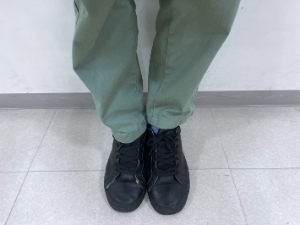
\includegraphics[keepaspectratio, scale=0.7] {images/RobotGuidance_following_phase_leg.png}
  \captionsetup{justification=raggedright} % キャプションを左寄せに
  \caption{Without retroreflective tape}
  \label{Fig:RobotGuidance_following_phase_leg}
\end{figure}

\begin{figure}[h]
  \centering
  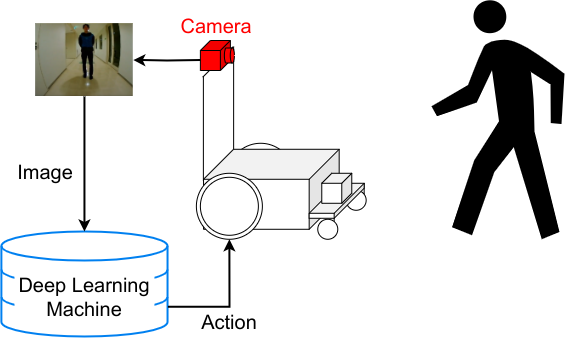
\includegraphics[keepaspectratio, scale=0.60] {images/RobotGuidance_following_system.png}
  \captionsetup{justification=raggedright} % キャプションを左寄せに
  \caption{Proposed method in the following phase}
  \label{Fig:RobotGuidance_following_system}
\end{figure}

\newpage
